\documentclass[a4paper]{article}
\usepackage[affil-it]{authblk}
\usepackage[backend=bibtex,style=numeric]{biblatex}
\usepackage{graphicx}

\usepackage{geometry}
\geometry{margin=1.5cm, vmargin={0pt,1cm}}
\setlength{\topmargin}{-1cm}
\setlength{\paperheight}{29.7cm}
\setlength{\textheight}{25.3cm}
\usepackage{listings}
\usepackage{color}
\definecolor{dkgreen}{rgb}{0,0.6,0}
\definecolor{gray}{rgb}{0.5,0.5,0.5}
\definecolor{mauve}{rgb}{0.58,0,0.82}

\lstset{ %
  language=c++,                % the language of the code
  basicstyle=\footnotesize,           % the size of the fonts that are used for the code
  numbers=left,                   % where to put the line-numbers
  numberstyle=\tiny\color{gray},  % the style that is used for the line-numbers
  stepnumber=2,                   % the step between two line-numbers. If it's 1, each line 
                                  % will be numbered
  numbersep=5pt,                  % how far the line-numbers are from the code
  backgroundcolor=\color{white},      % choose the background color. You must add \usepackage{color}
  showspaces=false,               % show spaces adding particular underscores
  showstringspaces=false,         % underline spaces within strings
  showtabs=false,                 % show tabs within strings adding particular underscores
  frame=single,                   % adds a frame around the code
  rulecolor=\color{black},        % if not set, the frame-color may be changed on line-breaks within not-black text (e.g. commens (green here))
  tabsize=2,                      % sets default tabsize to 2 spaces
  captionpos=b,                   % sets the caption-position to bottom
  breaklines=true,                % sets automatic line breaking
  breakatwhitespace=false,        % sets if automatic breaks should only happen at whitespace
  title=\lstname,                   % show the filename of files included with \lstinputlisting;
                                  % also try caption instead of title
  keywordstyle=\color{blue},          % keyword style
  commentstyle=\color{dkgreen},       % comment style
  stringstyle=\color{mauve},         % string literal style
  escapeinside={\%*}{*)},            % if you want to add LaTeX within your code
  morekeywords={*,...}               % if you want to add more keywords to the set
}

\begin{document}
% =================================================
\title{Report for Numerical Analysis programming homework \# 1}

\author{Shuo Chen 12231064
  \thanks{Email address: \texttt{shuo\_chen@zju.edu.cn}}}
\affil{(Electronic Science and Technology), Zhejiang University}



\date{Submitted time: \today}

\maketitle

\section*{A. Equation Solver}

Firstly, a base class \verb|EquationSolver| is created with a member \verb|function| and a virtual function \verb|solve|:
\begin{lstlisting}
class EquationSolver{
protected:
    const Function & F;
public:
    EquationSolver(const Function& F) : F(F){}
    virtual double solve() = 0;
};
\end{lstlisting}
Different methods are nothing more than derived classes of \verb|EquationSolver| with different \verb|solve| functions.
\subsection*{a. Bisection Method}
In the class \verb|Bisection_Method|, some parameters are set to control the accuracy and the maximum number of iterations. \verb|eps| stands for $\epsilon$, 
and \verb|delta| for $\delta$, which controls the accuracy of $f(x)$ and $x$ respectively. That means we find a root when $|f(x_{n+1})-f(x_n)| < \epsilon$ or $|x_{n+1}-x_n| < \delta$.

The iteration will continue if the conditions above is not satisfied until the maximum iterations. One of the ends of interval should be updated after each iteration. Assume that the interval is $[x_a,x_b]$ at a certain iteration with $x_{mid} = \frac{x_a + x_b}{2}$, 
if $f(x_a) * f(x_{mid}) > 0$, then the root is located in the interval $[x_{mid}, x_b]$, and the interval will be updated as $[x_a, x_{mid}]$ if $f(x_a) * f(x_{mid}) \leq 0$. The code is following according to the
ideas above.
\begin{lstlisting}
class Bisection_Method : public EquationSolver{
private:
    double a, b;
    double eps, delta;
    int Maxiter;
public:
    Bisection_Method(const Function& F, double a, double b, double eps = 1e-7, double delta = 1e-6, int Maxiter = 50):
        EquationSolver(F), a(a), b(b), eps(eps), delta(delta), Maxiter(Maxiter){}
    virtual double solve(){
        double h = b - a;
        double f_min_x = F(a);
        for(int i = 0; i < Maxiter; i++){
            h /= 2;
            double mid_x = a + h;
            if(h < delta){
                std::cout << "Iteration times: " << i << std::endl;
                std::cout << "Iteration stops for h < delta !" << std::endl;
                return mid_x;
            }
            double f_mid_x = F(mid_x);
            if(fabs(f_mid_x) < eps){
                std::cout << "Iteration times: " << i << std::endl;
                std::cout << "Iteration stops for fabs(f(x)) < eps !" << std::endl;
                return mid_x;
            }
            else if (f_min_x * f_mid_x > 0){
                a += h;
            }
        }
        std::cout << "Iteration times: " << Maxiter << std::endl;
        std::cout << "Iteration stops for reaching Maxiter !" << std::endl;
        return 0;
    }

};
\end{lstlisting}

\subsection*{b. Newton Method}
The iteration is changed into $x_{n+1} = x_n - \frac{f(x_n)}{f'(x_n)}$, with the same parameters in bisection method. The derivative of $f(x)$ is get by the \verb|derivative| function 
in the \verb|function| class.
\begin{lstlisting}
virtual double solve(){
    double x = x0;
    double f_x = F(x);
    for(int i = 0; i < Maxiter; i++){
        if(fabs(f_x) < eps){
            std::cout << "Iteration times: " << i << std::endl;
            std::cout << "Iteration stops for fabs(f(x)) < eps !" << std::endl;
            return x;
        }
        double d_fx = F.derivative(x0);
        x -= f_x / d_fx;
        f_x = F(x);
    }
    std::cout << "Iteration times: " << Maxiter << std::endl;
    std::cout << "Iteration stops for reaching Maxiter !" << std::endl;
    return 0;
}
\end{lstlisting}

\subsection*{c. Secant Method}
It is all the same with Newton method but the calculation of derivative. The difference is used instead of the direct derivative, therefore two points are used in 
each iteration, while only one point needed in Newton Method.
\begin{lstlisting}
virtual double solve(){
    double x_0 = x0;
    double x_1 = x1;
    double f_x0 = F(x0);
    double f_x1 = F(x1);
    for(int i = 0; i < Maxiter; i++){
        double x_dis = fabs(x_0 - x_1);
        if(x_dis < delta){
            std::cout << "Iteration times: " << i << std::endl;
            std::cout << "Iteration stops for |x_{n+1} - x_n| < delta !" << std::endl;
            return x_1;
        }
        if(fabs(f_x1) < eps){
            std::cout << "Iteration times: " << i << std::endl;
            std::cout << "Iteration stops for fabs(f(x)) < eps !" << std::endl;
            return x_1;
        }
        double df = (f_x0 - f_x1) / (x_0 - x_1);
        x_0 = x_1;
        x_1 = x_1 - f_x1 / df;
        f_x0 = F(x_0);
        f_x1 = F(x_1);
    }
    std::cout << "Iteration times: " << Maxiter << std::endl;
    std::cout << "Iteration stops for reaching Maxiter !" << std::endl;
    return 0;
}
\end{lstlisting}

\section*{B. Test for bisection method}
Just use the solvers in part A, with $\verb|eps| = 10^{-7}$, $\verb|delta| = 10^{-6}$, $\verb|Maxiter| = 50$. But there is something need to pay attetion to:

In the first question, $f(x) = x^{-1} - \tan x$ with the interval $[0,\frac{\pi}{2}]$. $f$ is not defined at $0$ and $\frac{\pi}{2}$, which is not satisfied the 
precondition of bisection method. However, $\lim_{x\rightarrow 0^+}f(x) = +\infty$, $\lim_{x\rightarrow \frac{\pi}{2}^-}f(x) = -\infty$, and $f$ is continuous, so there must be 
a root in $(0,\frac{\pi}{2})$.

Therefore, we add a perturbation at the ends of the interval, which means we changed the interval into $[\Delta_x, \frac{\pi}{2} - \Delta_x]$. We noticed that $f(x)$ 
is monotonically decreasing on $(0,\frac{\pi}{2})$. If $\Delta_x$ is small 
enough to guarantee $f(x) > 0$ on $(0,\Delta_x)$ and $f(x) < 0$ on $(\frac{\pi}{2} - \Delta_x, \frac{\pi}{2})$, the root would not be omitted.

Similar case is also in the second question, which can be solved by the same trick.

Here is result of 4 equations:
\begin{table}[!ht]
    \centering
    \begin{tabular}{|l|l|l|l|l|l|}
    \hline
        ~ & Initial Interval& Root & Iteration Times & Why Iteration Stops & Remark \\ \hline
        $x^{-1} - \tan x$ & $[0,\frac{\pi}{2}]$ & 0.860333 & 20 & $|x_{n+1}-x_n| < \delta$ & $\Delta_x = 10^{-7}$ \\ \hline
        $x^{-1} - 2^x$ & $[0,1]$ & 0.641186 & 17 & $|f(x)| < \epsilon$ & $\Delta_x = 10^{-7}$ \\ \hline
        $2^{-x} + e^{x} + 2\cos{x} - 6$ & $[1,3]$ & 1.82938 & 20 & $|x_{n+1}-x_n| < \delta$ & ~ \\ \hline
        $\frac{(x^3 + 4x^2 + 3x + 5)}{(2x^3 - 9x^2 + 18x - 2)}$ & $[0,4]$ & 0.117877 & 21 & $|x_{n+1}-x_n| < \delta$ & ~ \\ \hline
    \end{tabular}
\end{table}

\section*{C. Test for Newton Method}
Just use the solvers in part A, with $\verb|eps| = 10^{-7}$, $\verb|delta| = 10^{-6}$, $\verb|Maxiter| = 50$.

Here is the result:
\begin{table}[!ht]
    \centering
    \begin{tabular}{|l|l|l|l|l|}
    \hline
        ~ & Initial Value& Root & Iteration Times & Why Iteration Stops\\ \hline
        $x - \tan x$ & 4.5 & 4.49341 & 5 & $|f(x)| < \epsilon$ \\ \hline
        $x - \tan x$ & 7.7 & 7.72525 & 20 & $|f(x)| < \epsilon$ \\ \hline
    \end{tabular}
\end{table}

\section*{D. Test for Secant Method}
Just use the solvers in part A, with $\verb|eps| = 10^{-7}$, $\verb|delta| = 10^{-6}$, $\verb|Maxiter| = 50$. It is noticed that each equation has multiple roots,
 so there could be different results with different initial values.

Two kinds of initial values are given in each case to get different roots, which implies the algorithm is deeply influenced by the selection of initial value.

Here is the result:
\begin{table}[!ht]
    \centering
    \begin{tabular}{|l|l|l|l|l|}
    \hline
        ~ & Initial Value& Root & Iteration Times & Why Iteration Stops\\ \hline
        $\sin(\frac{x}{2}) - 1$ & $0,\frac{\pi}{2}$ & 3.14093 & 16 & $|f(x)| < \epsilon$ \\ \hline
        $\sin(\frac{x}{2}) - 1$ & $2\pi,\frac{9\pi}{2}$ & 15.7073 & 16 & $|f(x)| < \epsilon$ \\ \hline
        $e^{x} - \tan x$ & $1,1.4$ & 1.30633 & 9 & $|x_{n+1} - x_n| < \delta$ \\ \hline
        $e^{x} - \tan x$ & $10,11$ & -3.09641 & 25 & $|f(x)| < \epsilon$ \\ \hline
        $x^3 - 12x^2 + 3x + 1$ & $0,-0.5$ & -0.188685 & 6 & $|f(x)| < \epsilon$ \\ \hline
        $x^3 - 12x^2 + 3x + 1$ & $10,11$ & 11.7371 & 6 & $|f(x)| < \epsilon$ \\ \hline
    \end{tabular}
\end{table}

\section*{E. Fill the trough}

There is a formula which decribes the relation of $V$, $L$ ,$h$, and $r$. The question is to solve h, given the value of other parameters. It can be seen as a 
root-seek question, and 3 methods above can be used. Due to the derivative of $h$ is not easy to calculate, I take the bisection method for the reason that $V$ 
is a monotonically increasing function of $h$, and the root should be in $(0, r)$ to make it reasonable.

Here is the result:
\begin{table}[!ht]
    \centering
    \begin{tabular}{|l|l|l|l|l|}
    \hline
        ~ & Initial Interval& Root & Iteration Times & Why Iteration Stops\\ \hline
        $V(h)$ & $[0,r]$ & 0.1665161 & 6 & $|f(x)| < \epsilon$ \\ \hline
    \end{tabular}
\end{table}

\section*{F. Nose-in failure of a vehicle}

Problem (a) and (b) can be solved just using Newton method with given parameters, and here is the result:

\begin{table}[!ht]
    \centering
    \begin{tabular}{|l|l|l|l|l|}
    \hline
        ~ & Initial Value& Root & Iteration Times & Why Iteration Stops\\ \hline
        $D = 55$ & 33 & 32.9722 & 2 & $|f(x)| < \epsilon$ \\ \hline
        $D = 30$ & 33 & 33.1689 & 2 & $|f(x)| < \epsilon$ \\ \hline
    \end{tabular}
\end{table}

Secant method is used in problem (c) with different initial values, and here is the result(with $D = 30$):

\begin{table}[!ht]
    \centering
    \begin{tabular}{|l|l|l|l|}
    \hline
        Initial Value& Root & Iteration Times & Why Iteration Stops\\ \hline
        30, 60& 33.1689 & 4 & $|f(x)| < \epsilon$ \\ \hline
        0, 10& -11.5 & 8 & $|f(x)| < \epsilon$ \\ \hline
        80, 90& -10451.5 & 19 & $|f(x)| < \epsilon$ \\ \hline
    \end{tabular}
\end{table}

It is easily observed that results changed enormously with different initial values. To see it more clearly, I print the function image on $[0,360]$(one period):
\begin{figure}[h]
    \centering
    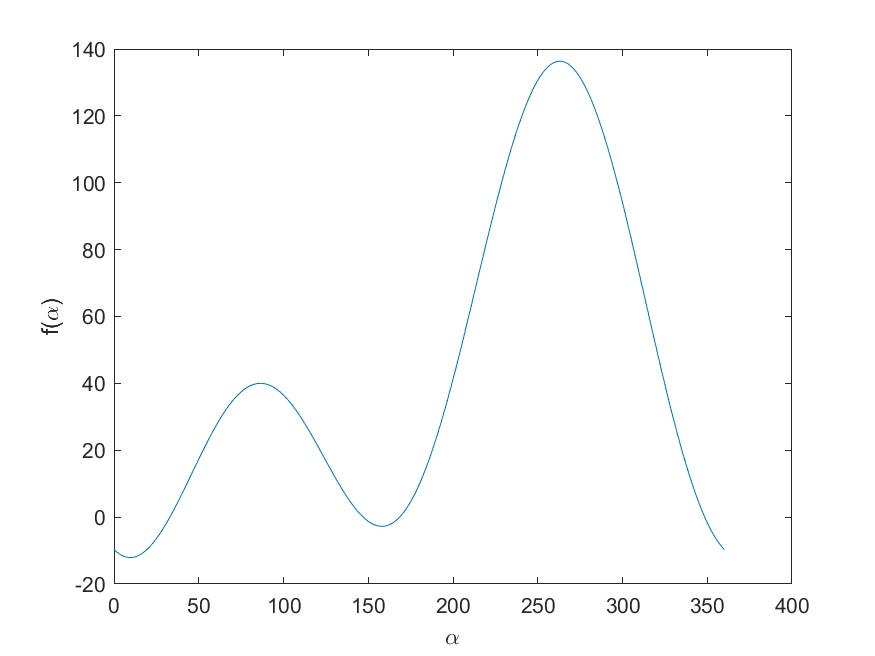
\includegraphics[width=0.5\textwidth]{fig/ProblemF.jpg}
    \caption{ProblemF}
    \label{fig:ProblemF}
\end{figure}

It is illustrated that there is a root near 33, while another two roots near 150 and 350. In addition, this function is periodic, which means $f(x+360) = 0$ if $f(x) = 0$.

Therefore, if the initial value is different, the result can run everywhere depends on the algorithm.

\end{document}